%%%%%%%%%%%%%%%%%%% EJERCICIO 1 %%%%%%
\textbf{Ejemplo 1:}\\

Se va a cancelar una deuda por 200.000 COP en 4 pagos trimestrales de R COP cuota ordinaria, con una tasa de interés de 32\% nominal anual trimestre vencido. Hallar el valor de las cuotas ordinarias.\\

\textbf{Ejemplo 1:}\\
Tenemos un capital de 200{.}000 COP que será invertido al 10\% 
periódico trimestre vencido (ptv), durante un año. Use año de 360 días.\\

A. Calcular el valor total de los intereses simples, si:
\begin{itemize}
  \item son cancelados cada trimestre.
  \item son capitalizados y cancelados al final del tiempo de la inversión.
\end{itemize}
B. ¿A qué tasa de interés periódica año vencido (pav) es equivalente la tasa de 10\% 
periódica trimestre vencido (ptv)?\\

%%%%%%%%%%%%%%%%%%% EJERCICIO 1 %%%%%%

%\newpage %USAR SOLO SI EL SOLUCIÓN QUEDA SOLO Y ES NECESARIO BAJARLO A LA SIGUIENTE PAGINA
\textbf{Solución.}\\

%La tabla ira centrada
\begin{center}
  \renewcommand{\arraystretch}{1.5}% Margenes de las celdas
  %Creación de la cuadricula de 3 columnas
  \begin{flushleft}\textbf{A.1} \end{flushleft}
  \begin{longtable}[H]{|C{0.3\linewidth}|C{0.3\linewidth}|C{0.3\linewidth}|}
    %Creamos una linea horizontal
    \hline
    %Definimos el color de la primera fila
    \rowcolor[HTML]{FFB183}
    %%%%% INICIO ASIGNACIÓN PERIODO FOCAL %%%%%%%
    %%%%%%%%%% INICIO TITULO
    %Lo que se hace aquí es mezclar las 3 columnas en una sola
    \multicolumn{3}{|c|}{\cellcolor[HTML]{FFB183}\textbf{1. Asignación período focal}} \\ \hline
    %%%%%%%%%% FIN TITULO
    %%%%% INICIO DECLARACIÓN DE VARIABLES %%%%%%%
    \multicolumn{3}{|c|}{$pf = 4ptv$}  \\ \hline
    %%%%%%%%%% INICIO TITULO
    %Lo que se hace aquí es mezclar las 3 columnas en una sola
    \multicolumn{3}{|c|}{\cellcolor[HTML]{FFB183}\textbf{2. Declaración de variables}}  \\ \hline
    %%%%%%%%%% FIN TITULO
    %%%%%%%%%% INICIO DE MATEMÁTICAS
    %Cada & hace referencia al paso de la siguiente columna
    $P =  200{.}000 COP$ & $i = 10\%\textit{ ptv} $  & $I= ? COP$  \\
      & $n=\frac{90 dias}{90dias} =1 ptv$  & $F= ? COP$
    \\\hline

    %%%%%%%%%% FIN DE MATEMÁTICAS
    %%%%% FIN DECLARACIÓN DE VARIABLES


    %%%%% INICIO FLUJO DE CAJA
    \rowcolor[HTML]{FFB183}
    \multicolumn{3}{|c|}{\cellcolor[HTML]{FFB183}\textbf{3. Diagrama de flujo de caja}}  \\ \hline
    %Mezclamos 3 columnas y podremos el dibujo
    %%%%%%%%%%%%% INSERCIÓN DE LA IMAGEN
    %Deberán descargar las imágenes respectivas del drive y pegarlas en la carpeta
    %n_capitulo/img/ejemplos/1/capitulo1ejemplo1.pdf  (el /1/ es el numero del ejemplo)
    \multicolumn{3}{|c|}{ 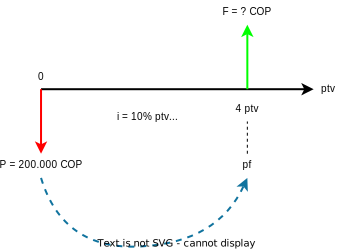
\includegraphics[trim=-5 -5 -5 -5 , scale=1]{2_Capitulo/ejemplos/1/Capitulo2Ejercicio1a_v2.pdf} }  \\ \hline
    %%%%%%%%%%%%% FIN INSERCIÓN DE IMAGEN
    %%%%%FIN FLUJO DE CAJA



    %%%%% INICIO DECLARACIÓN FORMULAS
    %%%%%%%%%%% INICIO TITULO
    \rowcolor[HTML]{FFB183}
    \multicolumn{3}{|c|}{\cellcolor[HTML]{FFB183}\textbf{4. Declaración de fórmulas}}  \\ \hline
    %%%%%%%%%%% FIN TITULO
    %%%%%%%%%%% INICIO MATEMÁTICAS

    $I = Pin\hspace{0.3cm} \textit{Interés monetario simple}$ & \multicolumn{2}{c|}{$F = P + I \hspace{0.3cm} \textit{Valor futuro}$}                 \\ \hline
    %%%%%%%%%% FIN MATEMÁTICAS
    %%%%%% INICIO DESARROLLO MATEMÁTICO
    \rowcolor[HTML]{FFB183}
    %%%%%%%%%%INICIO TITULO
    \multicolumn{3}{|c|}{\cellcolor[HTML]{FFB183}\textbf{5. Desarrollo matemático}}                                                                   \\ \hline
    %%%%%%%%%% FIN TITULO
    %%%%%%%%%% INICIO MATEMÁTICAS
    \multicolumn{3}{|c|}{$I_{1}= (200.000 COP)(0.1)(1)$}                                                                                             \\ \multicolumn{3}{|c|}{$I_{1}=   20{.}000 COP$}  \\ \multicolumn{3}{|c|}{$I_{1} = I_{2} = I_{3} = I_{4}$}  \\
    \multicolumn{3}{|c|}{$I = (4)(20.000 COP) =  80.000 COP$}                                                                                       \\ \multicolumn{3}{|c|}{$F = P + I$} \\ \multicolumn{3}{|c|}{$F = 200{.}000 COP +  80{.}000 COP =  280{.}000 COP$} \\ \hline


    %%%%%%%%%% FIN MATEMÁTICAS
    %%%%%% FIN DESARROLLO MATEMÁTICO
    %%%%%% INICIO RESPUESTA
    \rowcolor[HTML]{FFB183}
    %%%%%%%%%%INICIO TITULO
    \multicolumn{3}{|c|}{\cellcolor[HTML]{FFB183}\textbf{6. Respuesta}}                                                                               \\ \hline
    %%%%%%%%%% FIN TITULO
    %%%%%%%%%% INICIO RESPUESTA MATEMÁTICA
    $I= 80{.}000 COP$                                        &
    \multicolumn{2}{c|}{$F= 280{.}000 COP$
    }                                                                                                                                                 \\ \hline
    %%%%%%%%%% FIN MATEMÁTICA
    %%%%%% FIN RESPUESTA
  \end{longtable}
  %Se crean dos lineas en blanco para que no quede el siguiente texto tan pegado
  %\newline \newline %USARLO SI CREES QUE ES NECESARIO
\end{center}
%%%%%%%%%%%%%%%%%%%%%%%%%%FIN EJERCICIO 1 %%%%%%%%%%%%%%%%%%%%%%%%%%%


%%%%%%%%%%%%%%%%%%% EJERCICIO 1 %%%%%%

%\newpage %USAR SOLO SI EL SOLUCIÓN QUEDA SOLO Y ES NECESARIO BAJARLO A LA SIGUIENTE PAGINA

%La tabla ira centrada
\begin{center}
  \renewcommand{\arraystretch}{1.5}% Margenes de las celdas
  %Creación de la cuadricula de 3 columnas
  \begin{flushleft}\textbf{A.2} \end{flushleft}
  \begin{longtable}[H]{|C{0.3\linewidth}|C{0.3\linewidth}|C{0.3\linewidth}|}
    %Creamos una linea horizontal
    \hline
    %Definimos el color de la primera fila
    \rowcolor[HTML]{FFB183}
    %%%%% INICIO ASIGNACIÓN FECHA FOCAL %%%%%%%
    %%%%%%%%%% INICIO TITULO
    %Lo que se hace aquí es mezclar las 3 columnas en una sola
    \multicolumn{3}{|c|}{\cellcolor[HTML]{FFB183}\textbf{1. Asignación período focal}}  \\ \hline
    %%%%%%%%%% FIN TITULO
    %%%%% INICIO DECLARACIÓN DE VARIABLES %%%%%%%
    \multicolumn{3}{|c|}{$pf = 4ptv$} \\ \hline
    %%%%%%%%%% INICIO TITULO
    %Lo que se hace aquí es mezclar las 3 columnas en una sola
    \multicolumn{3}{|c|}{\cellcolor[HTML]{FFB183}\textbf{2. Declaración de variables}}  \\ \hline
    %%%%%%%%%% FIN TITULO
    %%%%%%%%%% INICIO DE MATEMÁTICAS
    %Cada & hace referencia al paso de la siguiente columna
    
    $P =  200{.}000 COP$  & $i = 10\%\textit{ ptv} $  & $I= ? COP$   \\
      & $n=\frac{360 \textit{días}}{90 \textit{días}} =4 ptv$ & $F= ? COP$
    \\\hline

    %%%%%%%%%% FIN DE MATEMÁTICAS
    %%%%% FIN DECLARACIÓN DE VARIABLES

    %%%%% INICIO FLUJO DE CAJA
    \rowcolor[HTML]{FFB183}
    \multicolumn{3}{|c|}{\cellcolor[HTML]{FFB183}\textbf{3. Diagrama de flujo de caja}}                                                                          \\ \hline
    %Mezclamos 3 columnas y pondremos el dibujo
    %%%%%%%%%%%%% INSERCIÓN DE LA IMAGEN
    %Deberán descargar las imágenes respectivas del drive y pegarlas en la carpeta
    %n_capitulo/img/ejemplos/1/capitulo1ejemplo1.pdf  (el /1/ es el numero del ejemplo)
    \multicolumn{3}{|c|}{ 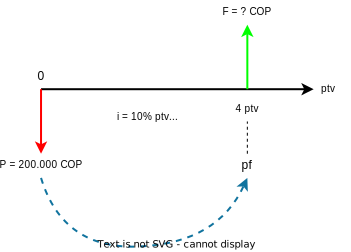
\includegraphics[trim=-5 -5 -5 -5 , scale=1]{2_Capitulo/ejemplos/1/Capitulo2Ejercicio1a2_v2.pdf} }                                         \\ \hline
    %%%%%%%%%%%%% FIN INSERCIÓN DE IMAGEN
    %%%%%FIN FLUJO DE CAJA

    %%%%% INICIO DECLARACIÓN FORMULAS
    %%%%%%%%%%% INICIO TITULO
    \rowcolor[HTML]{FFB183}
    \multicolumn{3}{|c|}{\cellcolor[HTML]{FFB183}\textbf{4. Declaración de fórmulas}}                                                                            \\ \hline
    %%%%%%%%%%% FIN TITULO
    %%%%%%%%%%% INICIO MATEMÁTICAS

    $I = Pin\hspace{0.3cm} \textit{Interés monetario simple}$ & \multicolumn{2}{c|}{$F = P + I \hspace{0.3cm} \textit{Valor futuro}$}                            \\ \hline
    %%%%%%%%%% FIN MATEMÁTICAS
    %%%%%% INICIO DESARROLLO MATEMÁTICO
    \rowcolor[HTML]{FFB183}
    %%%%%%%%%%INICIO TITULO
    \multicolumn{3}{|c|}{\cellcolor[HTML]{FFB183}\textbf{5. Desarrollo matemático}}                                                                              \\ \hline
    %%%%%%%%%% FIN TITULO
    %%%%%%%%%% INICIO MATEMÁTICAS
    $n=4ptv$                                                  & \multicolumn{2}{c|}{}                                                                            \\ $I_{1}= 200{.}000$ COP$\cdot0.1\cdot1$ & \multicolumn{2}{c|}{$F =  200{.}000$ COP + $20{.}000$ COP + $22{.}000$ COP}  \\ $I_{1}=  20{.}000$ COP & \multicolumn{2}{c|}{$+ 24{.}200$ COP + $26{.}620$ COP}  \\
    $I_{2}= 220{.}000\cdot0.1\cdot1$ COP   & \multicolumn{2}{c|}{$F= P+I$} \\
    $I_{2}= 22{.}000$ COP                  & \multicolumn{2}{c|}{$F=200{.}000$ COP$+92{.}820$ COP}   \\
    $I_{3}= 242{.}000\cdot0.1\cdot1$ COP   & \multicolumn{2}{c|}{$F= 292{.}820$ COP}                \\
    $I_{3}= 24{.}200$ COP                  & \multicolumn{2}{c|}{}                                                           \\
    $I_{4}= 266{.}200\cdot0.1\cdot1$ COP   & \multicolumn{2}{c|}{}                                                                            \\
    $I_{4}= 26{.}620$ COP                  & \multicolumn{2}{c|}{}                                                                            \\
    $I= 20{.}000 COP + 22{.}000 COP + 24{.}200 COP + 26{.}620 COP$& \multicolumn{2}{c|}{}                                        \\
    $I= 92{.}820$ COP                      & \multicolumn{2}{c|}{}
    
    \\ \hline
    %%%%%%%%%% FIN MATEMÁTICAS
    %%%%%% FIN DESARROLLO MATEMÁTICO
    %%%%%% INICIO RESPUESTA
    \rowcolor[HTML]{FFB183}
    %%%%%%%%%%INICIO TITULO
    \multicolumn{3}{|c|}{\cellcolor[HTML]{FFB183}\textbf{6. Respuesta}}                                                                                          \\ \hline
    %%%%%%%%%% FIN TITULO
    %%%%%%%%%% INICIO RESPUESTA MATEMÁTICA
    $I= 92{.}820 COP$                                         &
    \multicolumn{2}{c|}{$F= 292{.}820 COP$
    }                                                                                                                                                            \\ \hline
    %%%%%%%%%% FIN MATEMÁTICAS
    %%%%%% FIN RESPUESTA
  \end{longtable}
  %Se crean dos lineas en blanco para que no quede el siguiente texto tan pegado
  %\newline \newline %USARLO SI CREES QUE ES NECESARIO
\end{center}
%%%%%%%%%%%%%%%%%%%%%%%%%%FIN EJERCICIO 1 %%%%%%%%%%%%%%%%%%%%%%%%%%%



Al elaborar la tabla de amortización, se debe tener presente que en el período 3 el valor del pago debe ser igual al pago ordinario más el pago extraordinario, tal como se ve en la siguiente tabla:\\


\begin{spacing}{1.1}
	%\begin{center}
	\begin{tabular}{|p{1cm}|p{3cm}|p{3cm}|p{3cm}|p{3cm}|}
		\hline
		\textbf{PER\ (1)} & \textbf{SALDO DEUDA (2)=(2)-(5)} & \textbf{INTERESES  (3)=(2)(i)} & \textbf{PAGO\ (4)=R COP - L COP} & \textbf{AMORTIZACIÓN  (5)=(4)-(3)} \\ \hline                    0 &   200.000,00 \ COP & --------- & --------- & ---------\\ \hline
		1                 &  167.599,56 \ COP                     &  16.000,00 \ COP                    &   48.400,44 \ COP                &  32.400,44 \ COP                        \\ \hline
		2                 &  132.609,08 \ COP                     &   13.407,96 \ COP                    &   48.400,44 \ COP                 &  34.992,48 \ COP                        \\ \hline
		3                 &  44.815,21 \ COP                      &  10.608,57 \ COP                     &    98.400,44 \ COP                 &  87.791,87 \ COP                        \\ \hline
		4                 &  0,00 \ COP                           &  3.585,23 \ COP                      &   48.400,44 \ COP                &  44.815,21 \ COP                        \\ \hline
	\end{tabular}
	%\end{center}
\end{spacing}
%%%%%%%%%%%%%%%%%%%%%%%%%%FIN EJERCICIO 1 %%%%%%%%%%%%%%%%%%%%%%%%%%%